\documentclass[11pt, oneside, a4paper, ngerman, parskip=half, listof=totoc]{scrreprt}
% VOR DEM DRUCK: auf twoside, openright stellen, Layout überprüfen, Datum auf Deckblatt auf das Abgabedatum stellen, (Leseprobe) aus dem Deckblatt entfernen.

% VOR DER ABGABE: Eidesstattliche Versicherung unterschreiben, Code auf CD Brennen und in mindestens eine Arbeit anhängen (diese ist zu händigen an Herr Schippritt), Drucke einmal durchblättern und schauen ob die okay sind
\usepackage{scrhack} % This seems to fix some compatibility issues somehow, idk why tho... internals and stuff...
\usepackage[autooneside=false, automark]{scrlayer-scrpage} % IDK why, but if this is not included this project will just explode

% \usepackage[T1]{fontenc} % Only needed when pdflatex is used instead of lualatex or xelatex
% \usepackage[utf8]{inputenc} % Only needed when pdflatex is used instead of lualatex or xelatex

\usepackage[backref,style=apa,backend=biber]{biblatex} %Used for bibliography
\usepackage{babel} %Used for bibliography
\usepackage{fontspec} % Defining your own fonts (see \setmonofont etc. below)
\usepackage[onehalfspacing]{setspace} % Spacing between lines in a document
\usepackage{geometry} % Page layout (see \geometry below)
\usepackage{tikz} % Tikz - Drawing vector graphics via TeX
\usepackage[breaklinks]{hyperref} % Cross referencing commands -> hypertext links to other sections for example (see \hypersetup below)
\usepackage[acronym,toc]{glossaries} % For creating acronym, toc and glossaries
\usepackage{amsmath} % For displaying mathematic equations
\usepackage{xcolor} % For defining HEX Colors with labels (see \definecolor below)
\usepackage{pgfplots} % Plotting scientific / statistical data like spreadsheets
\usepackage{graphicx} % Good if you want a bit more control over your graphics
\usepackage{rotating} % Good if you have a big figure which should be displayed sideways so it fits (\sidewaysfigure for example)
\usepackage{minted} % Code Listings with beautiful Syntax Highlighting (needs Python with the pygments package installed)
\usepackage{caption} % Used to configure custom captions for e.g. custom listings, etc. (somehow listings are a pain and needs some configuration here and there...)
\usepackage{pgf-umlsd} % UML - Sequencediagram via TIKZ
\usepackage[babel,german=quotes]{csquotes} % German quotes for citation
\raggedbottom

\setsansfont{CMU Sans Serif}
\setmainfont{CMU Serif}
\setmonofont{JetBrainsMono}[  % JetBrainsMono has to be installed for this to work
  Path,
  Extension      = .ttf,
  UprightFont    = *-Regular,
  ItalicFont     = *-Italic,
  BoldFont       = *-Bold,
  BoldItalicFont = *-BoldItalic,
]

% Define color aliases with hex values to be precise regarding graphics display.
\definecolor{purpleCol}{HTML}{8D07F6}
\definecolor{blueCol}{HTML}{0029FA}
\definecolor{blackCol}{HTML}{3D3D3D}
\definecolor{orangeCol}{HTML}{CF8A1B}
\definecolor{greenCol}{HTML}{0DA84B}
\definecolor{cyanCol}{HTML}{06A8C4}
\definecolor{redCol}{HTML}{D92329}

% Define color aliases by simply mixing colors by percentage: green!20 means 20% of green, 80% white, green!20!black means 20% green, 80% black.
\colorlet{sdgreen}{green!20}
\colorlet{sdblue}{blue!20}
\colorlet{sdorange}{orange!20}

% When using dateplot, might have to be changed depending on your needs.
\usepgfplotslibrary{dateplot}
\pgfplotsset{compat=1.18} % Throws warnings if not used. Some backwards compatibility issues.

% adjusts the spacing after subsubsection and subsections (and also sections if you want as you can see below).
\RedeclareSectionCommand[afterskip=.1\parskip]{subsubsection}
\RedeclareSectionCommand[afterskip=.1\parskip]{subsection}
%\RedeclareSectionCommand[afterskip=.1\parskip]{section}

\newenvironment{longlisting}{\captionsetup{type=listing}}{} % Needed when pasting big chunks of Code into a listing environment which spans around multiple pages.
\renewcommand\listoflistingscaption{Codeverzeichnis} % So the list of Listings displays "Codeverzeichnis" instead of "Listings" or so.
\renewcommand\listingscaption{Code} % So the captions of the Listings are prefixed "Code 1: ..." "Code 2: ..." etc.
\providecommand*{\listingautorefname}{Code} % So \autoref knows what to write, when it's used. E.g.: \autoref(code:xyz) will result in "Code 1" in the text.

% Settings for Code listings with nice Syntax Highlighting
\setminted{
  autogobble,
  frame=lines,
  framesep=2mm,
  baselinestretch=1,
  fontsize=\scriptsize,
  linenos
}

% Configurations for minted so you don't have to include the source code you want to display in the TeX Code.
% later you can then for example use \mintedtsfile{RELATIVEPATHTOTSFILE} to read and display TypeScript code, written into a separate .ts file.
\newmintedfile[mintedgraphqlfile]{gql.py:GraphqlLexer -x}{frame=lines,linenos}
\newmintedfile[mintedyamlfile]{yaml}{frame=lines,linenos,breaklines}
\newmintedfile[minteddockerfile]{dockerfile}{frame=lines,linenos,breaklines}
\newmintedfile[mintednginxfile]{nginx}{frame=lines,linenos,breaklines}
\newmintedfile[mintedtsfile]{typescript}{frame=lines,linenos,breaklines}
\newmintedfile[mintedxmlfile]{xml}{frame=lines,linenos,breaklines}

% Setting page layout
\geometry{
 %showframe, % Remove comment if you want to see the current page layout
  top=3cm,
  right=3cm,
  bottom=5cm,
  left=3cm
}

% defining hyperlink behaviour and looks
\hypersetup{
    colorlinks=true,
    hidelinks, % Comment this out if you want colored links
    linkcolor={red!50!black},
    citecolor={blue!50!black},
    urlcolor={blue!80!black}
}
\addbibresource{literature.bib} % So biber etc. can interpret your literature meta data for citation

% Adding tikz libraries for later use
\usetikzlibrary{
    positioning,
    intersections,
    shapes.geometric,
    shapes.misc,
    automata,
    fit,
    decorations.pathreplacing,
    calc
}

%% ARGUMENTE:
% 1: Nodes for the convex hull
% 2: Radius for the convex hull
% 3: Label for the line- and curvepoints
% 4: lineposition of linepoints for that convex hull
% 5: curvepointposition1 of the first pair of curvepoints for that convex hull
% 6: curvepointposition2 of the second pair of curvepoints for that convex hull
\newcommand{\convexpath}[2]{
  [   
  create hullcoords/.code={
    \global\edef\namelist{#1}
    \foreach [count=\counter] \nodename in \namelist {
      \global\edef\numberofnodes{\counter}
      \coordinate (hullcoord\counter) at (\nodename);
    }
    \coordinate (hullcoord0) at (hullcoord\numberofnodes);
    \pgfmathtruncatemacro\lastnumber{\numberofnodes+1}
    \coordinate (hullcoord\lastnumber) at (hullcoord1);
  },
  create hullcoords
  ]
  ($(hullcoord1)!#2!-90:(hullcoord0)$)
  \foreach [
  evaluate=\currentnode as \previousnode using \currentnode-1,
  evaluate=\currentnode as \nextnode using \currentnode+1
  ] \currentnode in {1,...,\numberofnodes} {
    let \p1 = ($(hullcoord\currentnode) - (hullcoord\previousnode)$),
    \n1 = {atan2(\y1,\x1) + 90},
    \p2 = ($(hullcoord\nextnode) - (hullcoord\currentnode)$),
    \n2 = {atan2(\y2,\x2) + 90},
    \n{delta} = {Mod(\n2-\n1,360) - 360}
    in 
    {arc [start angle=\n1, delta angle=\n{delta}, radius=#2]}
    -- ($(hullcoord\nextnode)!#2!-90:(hullcoord\currentnode)$)
  }
} % Drawing a convex path around TIKZ Nodes, see https://tex.stackexchange.com/questions/27171/padded-boundary-of-convex-hull
\newenvironment{customlegend}[1][]{%
    \begingroup
    % inits/clears the lists (which might be populated from previous
    % axes):
    \csname pgfplots@init@cleared@structures\endcsname
    \pgfplotsset{#1}%
}{%
    % draws the legend:
    \csname pgfplots@createlegend\endcsname
    \endgroup
}%

% makes \addlegendimage available (typically only available within an
% axis environment):
\def\addlegendimage{\csname pgfplots@addlegendimage\endcsname}

%%--------------------------------

% definition to insert numbers
\pgfkeys{/pgfplots/number in legend/.style={%
        /pgfplots/legend image code/.code={%
            \node at (0.125,-0.0225){#1}; % <= changed x value
        },%
    },
}
\pgfplotsset{
every legend to name picture/.style={west}
} % Sadly idk anymore where i got this, but it's very useful to display a legend under a figure, e.g. to describe node connections in particular.

\pagestyle{scrheadings}
\clearpairofpagestyles
\ihead{\leftmark}
\ohead{\Ifstr{\leftmark}{\rightmark}{}{\rightmark}}
\ofoot*{\pagemark}
\setkomafont{pagehead}{\normalfont}
\chapter{XY}
\label{cha:xy} % include all glossary entries which are being used throughout the project

\begin{document}
    \begin{titlepage}
    \begin{center}
    
    
\includegraphics[width=0.5\textwidth]{res/img/hshl_logo.jpg}
    %\vspace*{.1cm}
    
    \Large
    \textbf{Konzeptionierung und Implementierung eines Remote-Controllers mithilfe einer Microservice-Architektur zur Remote-basierten Nutzung einer On-Premise Software am Beispiel von Royal Render}
    \vspace{0.4cm}
    
    \large
    \textbf{Bachelorarbeit}
    %\vspace{1cm}
    
    Hochschule Hamm-Lippstadt\\
    Computervisualistik und Design

    vorgelegt von
    \vspace{0.1cm}
    
    \textbf{Robin Dürhager}\\
    Matrikelnummer: 2150495
    \vspace{0.3cm}
    
    \textbf{Erstprüfer}\\
    Prof. Dr. Darius Schippritt
    \vspace{0.3cm}
    
    \textbf{Zweitprüfer}\\
    Prof. Stefan Albertz
    \vspace{0.3cm}

    \textbf{Drittprüfer}\\
    Holger Schönberger
    \vspace{0.3cm}
    
    %\today
    24. März 2020

    \end{center}
    \end{titlepage}

    \newpage
    \cleardoublepage % Cover of the Work (IMPORTANT: SET YOUR PERSONAL INFORMATION IN THERE)
    \pagenumbering{roman} % Begin of Tables of Contents
    \begin{spacing}{1.15}
        \tableofcontents
        \listoffigures
        \listoflistings
    \end{spacing}  % End of Tables of Contents
    \clearpage \cleardoublepage
    \pagenumbering{arabic}

    %%%%%%%%%%% START OF THE MAIN WORK %%%%%%%%%%%
    % In here you can include .tex files from different folders for better debugging an a little cleaner folder structure.
    \chapter{XY}
\label{cha:xy}
    %%%%%%%%%%% END OF THE MAIN WORK %%%%%%%%%%%

    \printglossary[title=Akronyme,type=\acronymtype]  % Print all acronyms in a nice format
    \printglossary[title=Glossar]  % Print the glossary in a nice format
    \printbibliography[heading=bibintoc, title={Literaturverzeichnis}]  % Print the bibliography in a nice format
    \cleardoublepage
    \newpage
\chapter*{}\label{ch:affidavit}
\addcontentsline{toc}{chapter}{Eidesstattliche Versicherung}

% \includegraphics[width=0.95\textwidth]{misc/oath/Eidesstattliche_Versicherung.pdf}
%
Name: <VORNAME NACHNAME STUDENT>\\
Matrikel-Nr.: <MATRIKELNUMMER>\\
Studiengang: <STUDIENGANG>\\
\\
Ich versichere hiermit, dass ich die vorliegende Arbeit selbstständig und nur unter Benutzung der angegebenen Literatur und Hilfsmittel angefertigt habe. Wörtlich übernommene Sätze und Satzteile sind als Zitate belegt, andere Anlehnungen hinsichtlich Aussage und Umfang unter Quellenangabe kenntlich gemacht. Die Arbeit hat in gleicher oder ähnlicher Form noch keiner Prüfungsbehörde vorgelegen und ist auch noch nicht veröffentlicht.

\vspace{2.5cm}
\noindent\begin{tabular}{ll}
\makebox[5cm]{\hrulefill} & \makebox[7cm]{\hrulefill}\\ Ort, Datum & Unterschrift
\end{tabular} % oath which has to be hand signed
    \newpage
    \cleardoublepage
    \appendix
    \chapter{Anhang}
    \label{apx}
    \cleardoublepage
    \begin{figure}[!ht]
  \vspace{.02\textheight}
  \centering
  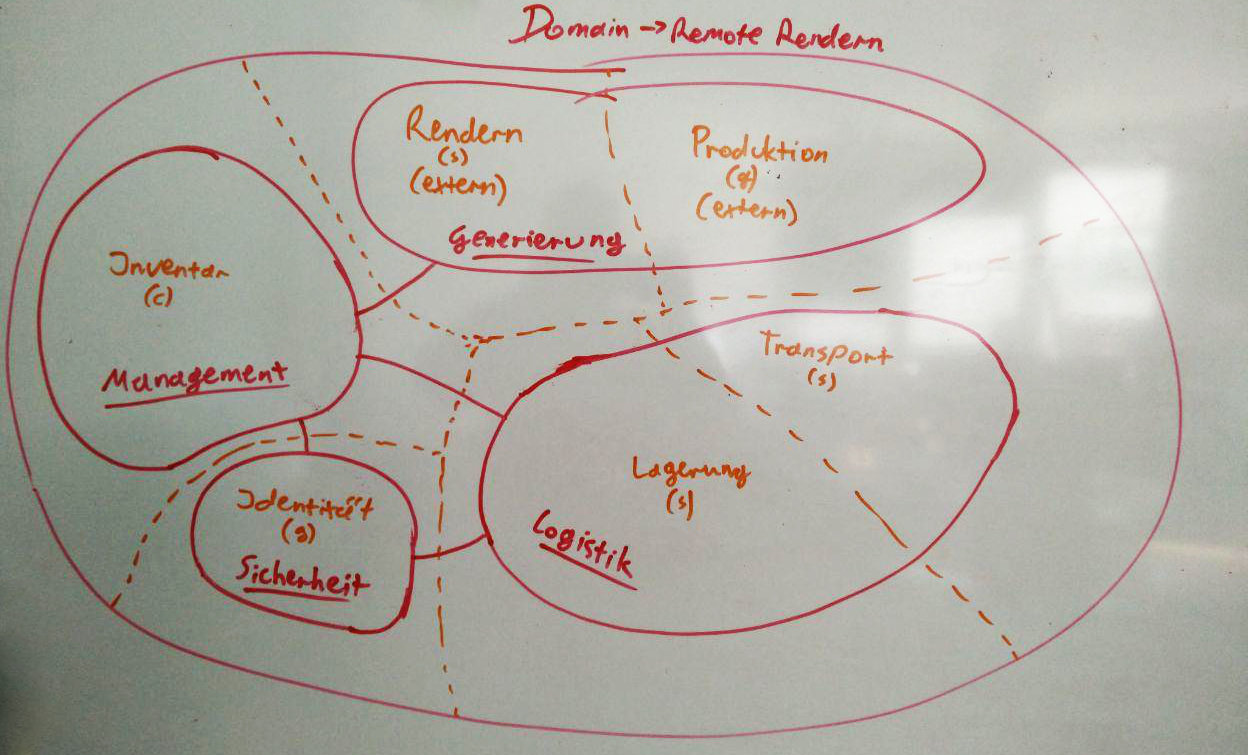
\includegraphics[width=\textwidth]{res/img/contextmap_rrRemote.jpg}
  \caption{Skizze der Kontextkarte der Domäne \emph{Remote Rendern}}
  \label{fig:drawing_contextmap_rrRemote}
\end{figure}
\clearpage

\begin{listing}[!ht]
  \vspace{.02\textheight}
  \mintedtsfile{./res/code/agw-willSendRequest.ts}
  \caption{Apollo Gateway Implementierung eines Sicherheitsmechanismus zur Absicherung gegen unautorisierte Zugriffe}
  \label{code:agw-security-function}
\end{listing}

\begin{sidewaysfigure}
  \centering
    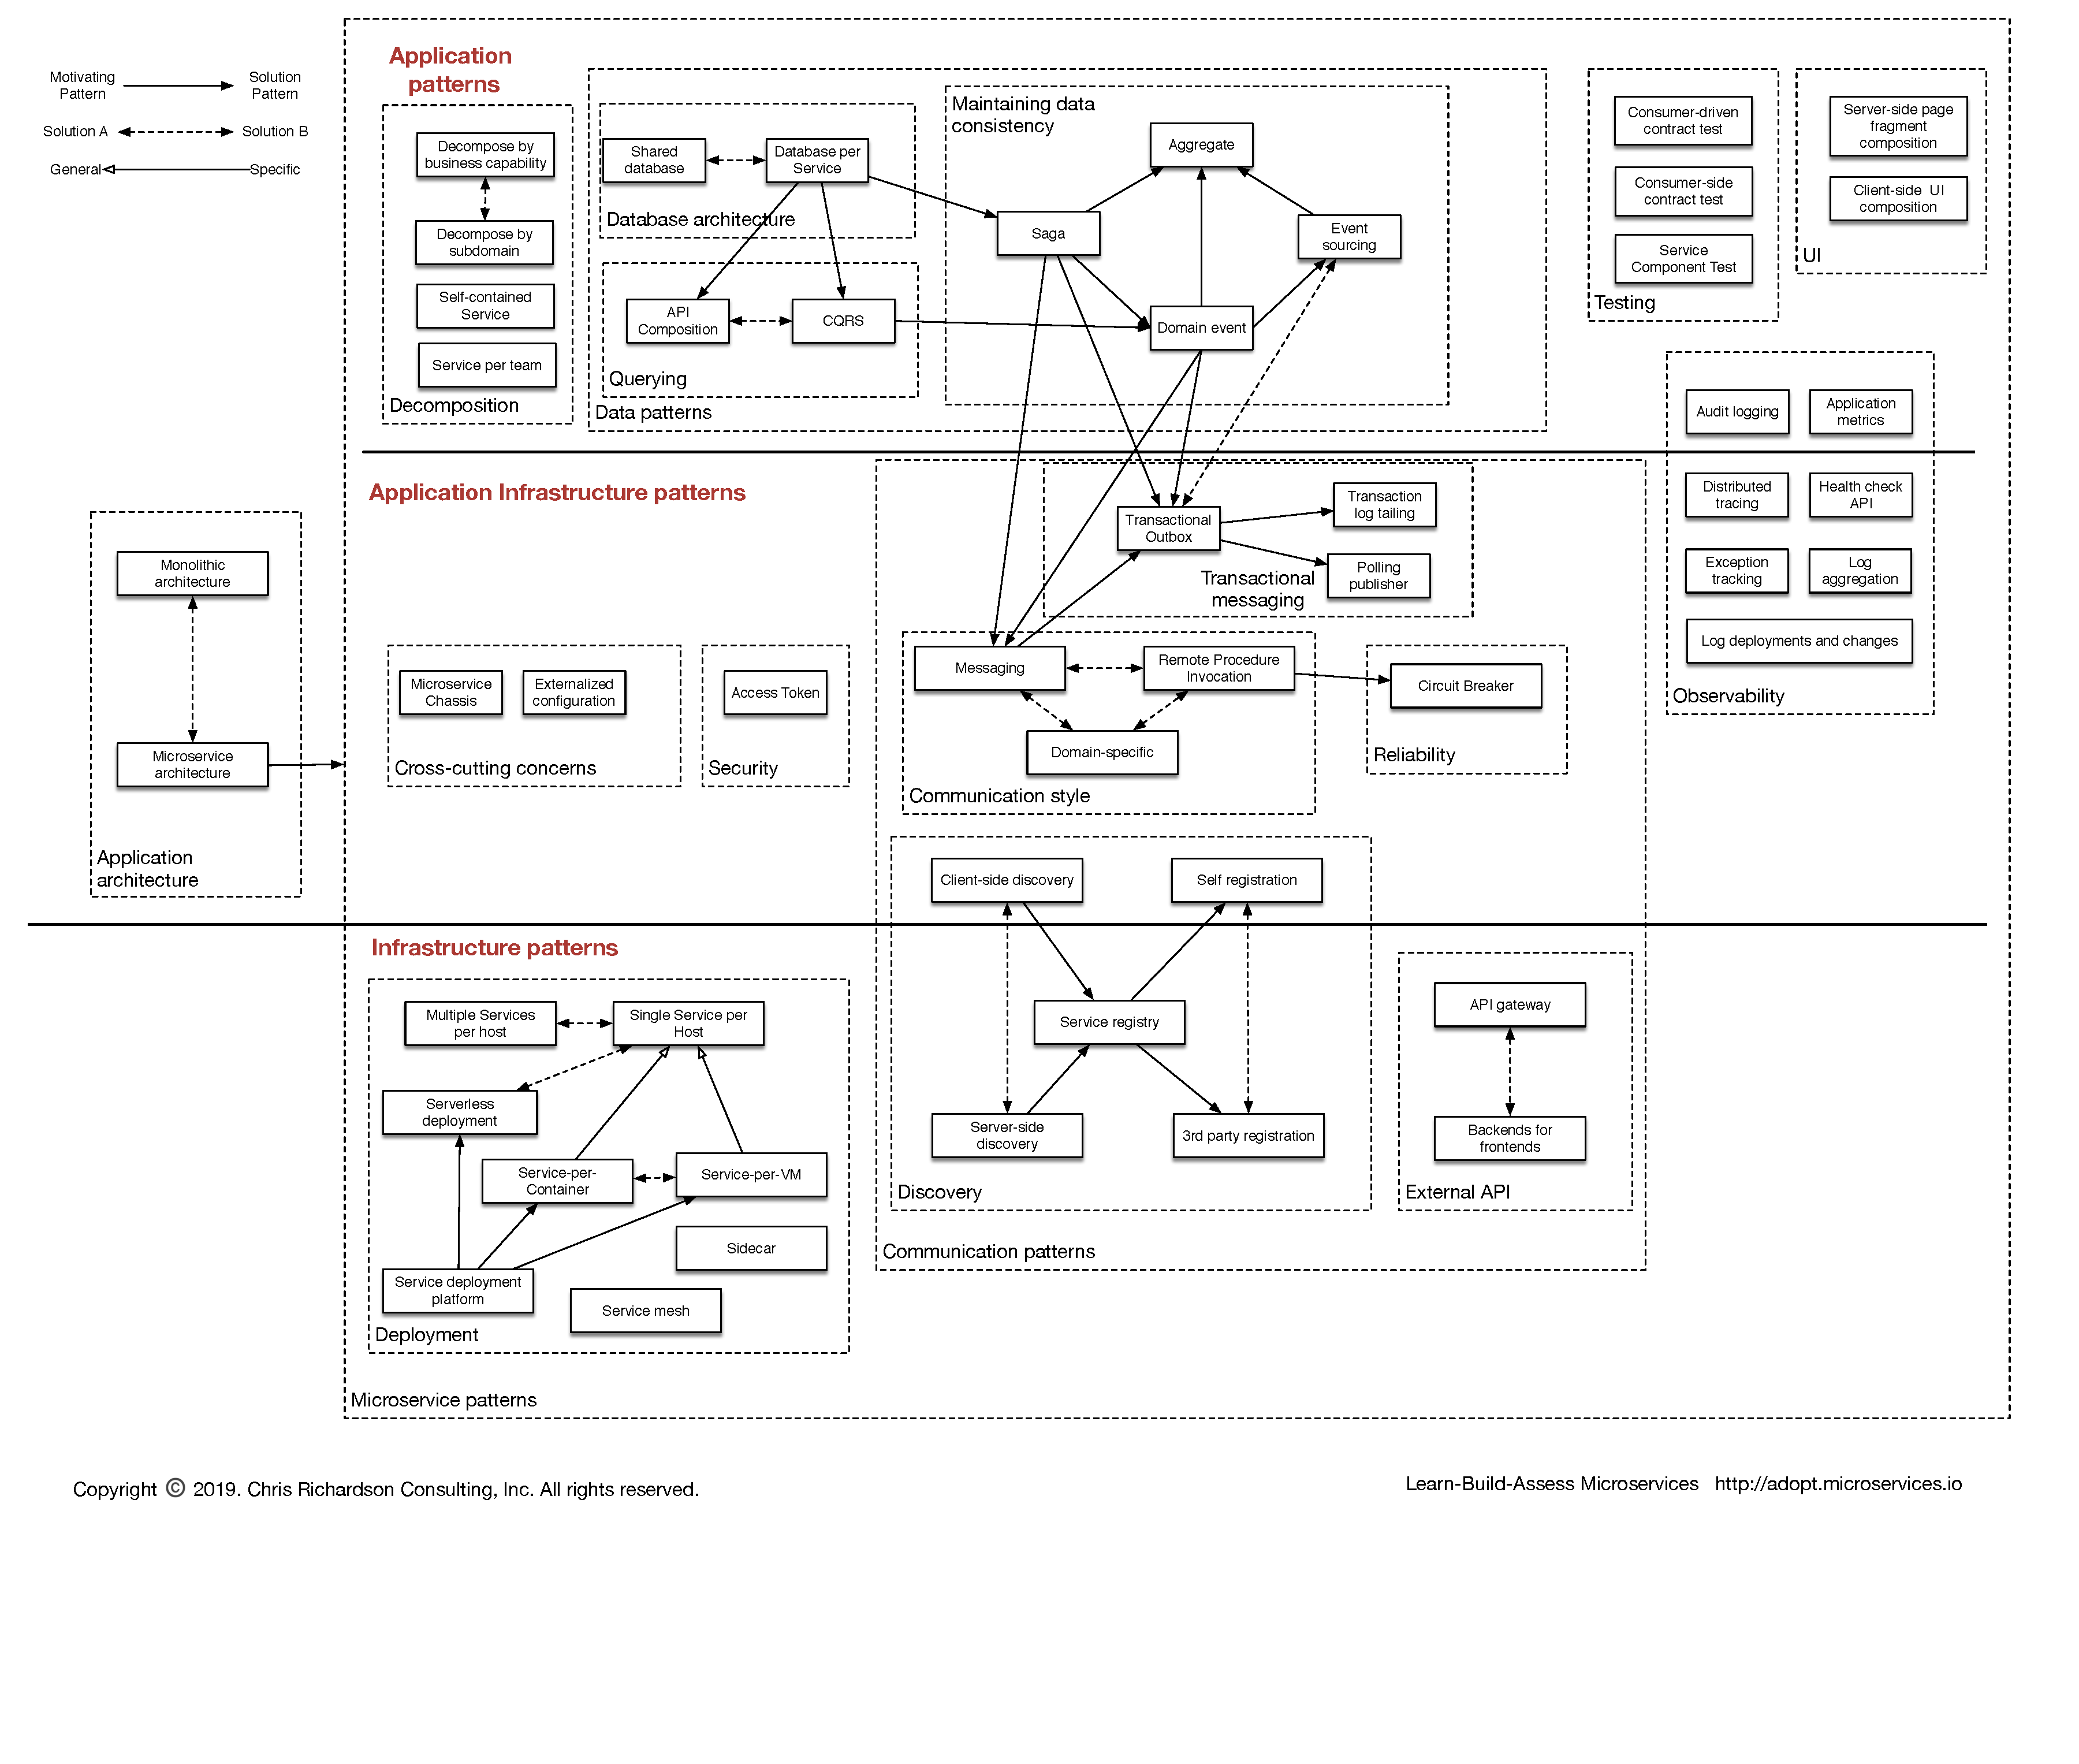
\includegraphics[width=\textwidth]{res/img/MicroservicePatternLanguage.pdf}
  \caption{Microservice Entwurfsmuster im Überblick \parencite{richardson2019mspatternlanguage}}
  \label{fig:microservice_patterns}
\end{sidewaysfigure}
\end{document}